\documentclass[10pt,a4paper]{article}

\usepackage{amsmath}
\usepackage{amsfonts}
\usepackage{amssymb}
\usepackage{graphicx}
\usepackage{float}
\usepackage{fullpage}
\usepackage{gensymb}
\usepackage{tabu}
\usepackage{tikz}
\usepackage{steinmetz} % allows for phasor notation with \phase{}

\newcommand*\circled[1]{\tikz[baseline=(char.base)]{
            \node[shape=circle,draw,inner sep=2pt] (char) {#1};}}

\author{David Lynch - 758863, Daniel Landgraf - 695683, Zixiang Ren }
\title{\huge{Electrical Network Analysis and Design} \\ Assignment 2}
\date{\small{Tuesday 2:15pm - EDS 8}}
\begin{document}
\maketitle

	\begin{enumerate}
		\item{
		%Question 1
		\let\clearpage\relax
		\def \sx {12500}
\def \sy {200000}
\def \sz {3.125\times 10^{10}}
\def \sw {50000}

\def \sa {\dfrac{13}{2500000}}
\def \sb {\dfrac{2}{25}}
\def \sc {50000}

\begin{enumerate}
	\item{
	%Part a
	\text{ }
		\begin{figure}[H]
		\begin{center}
		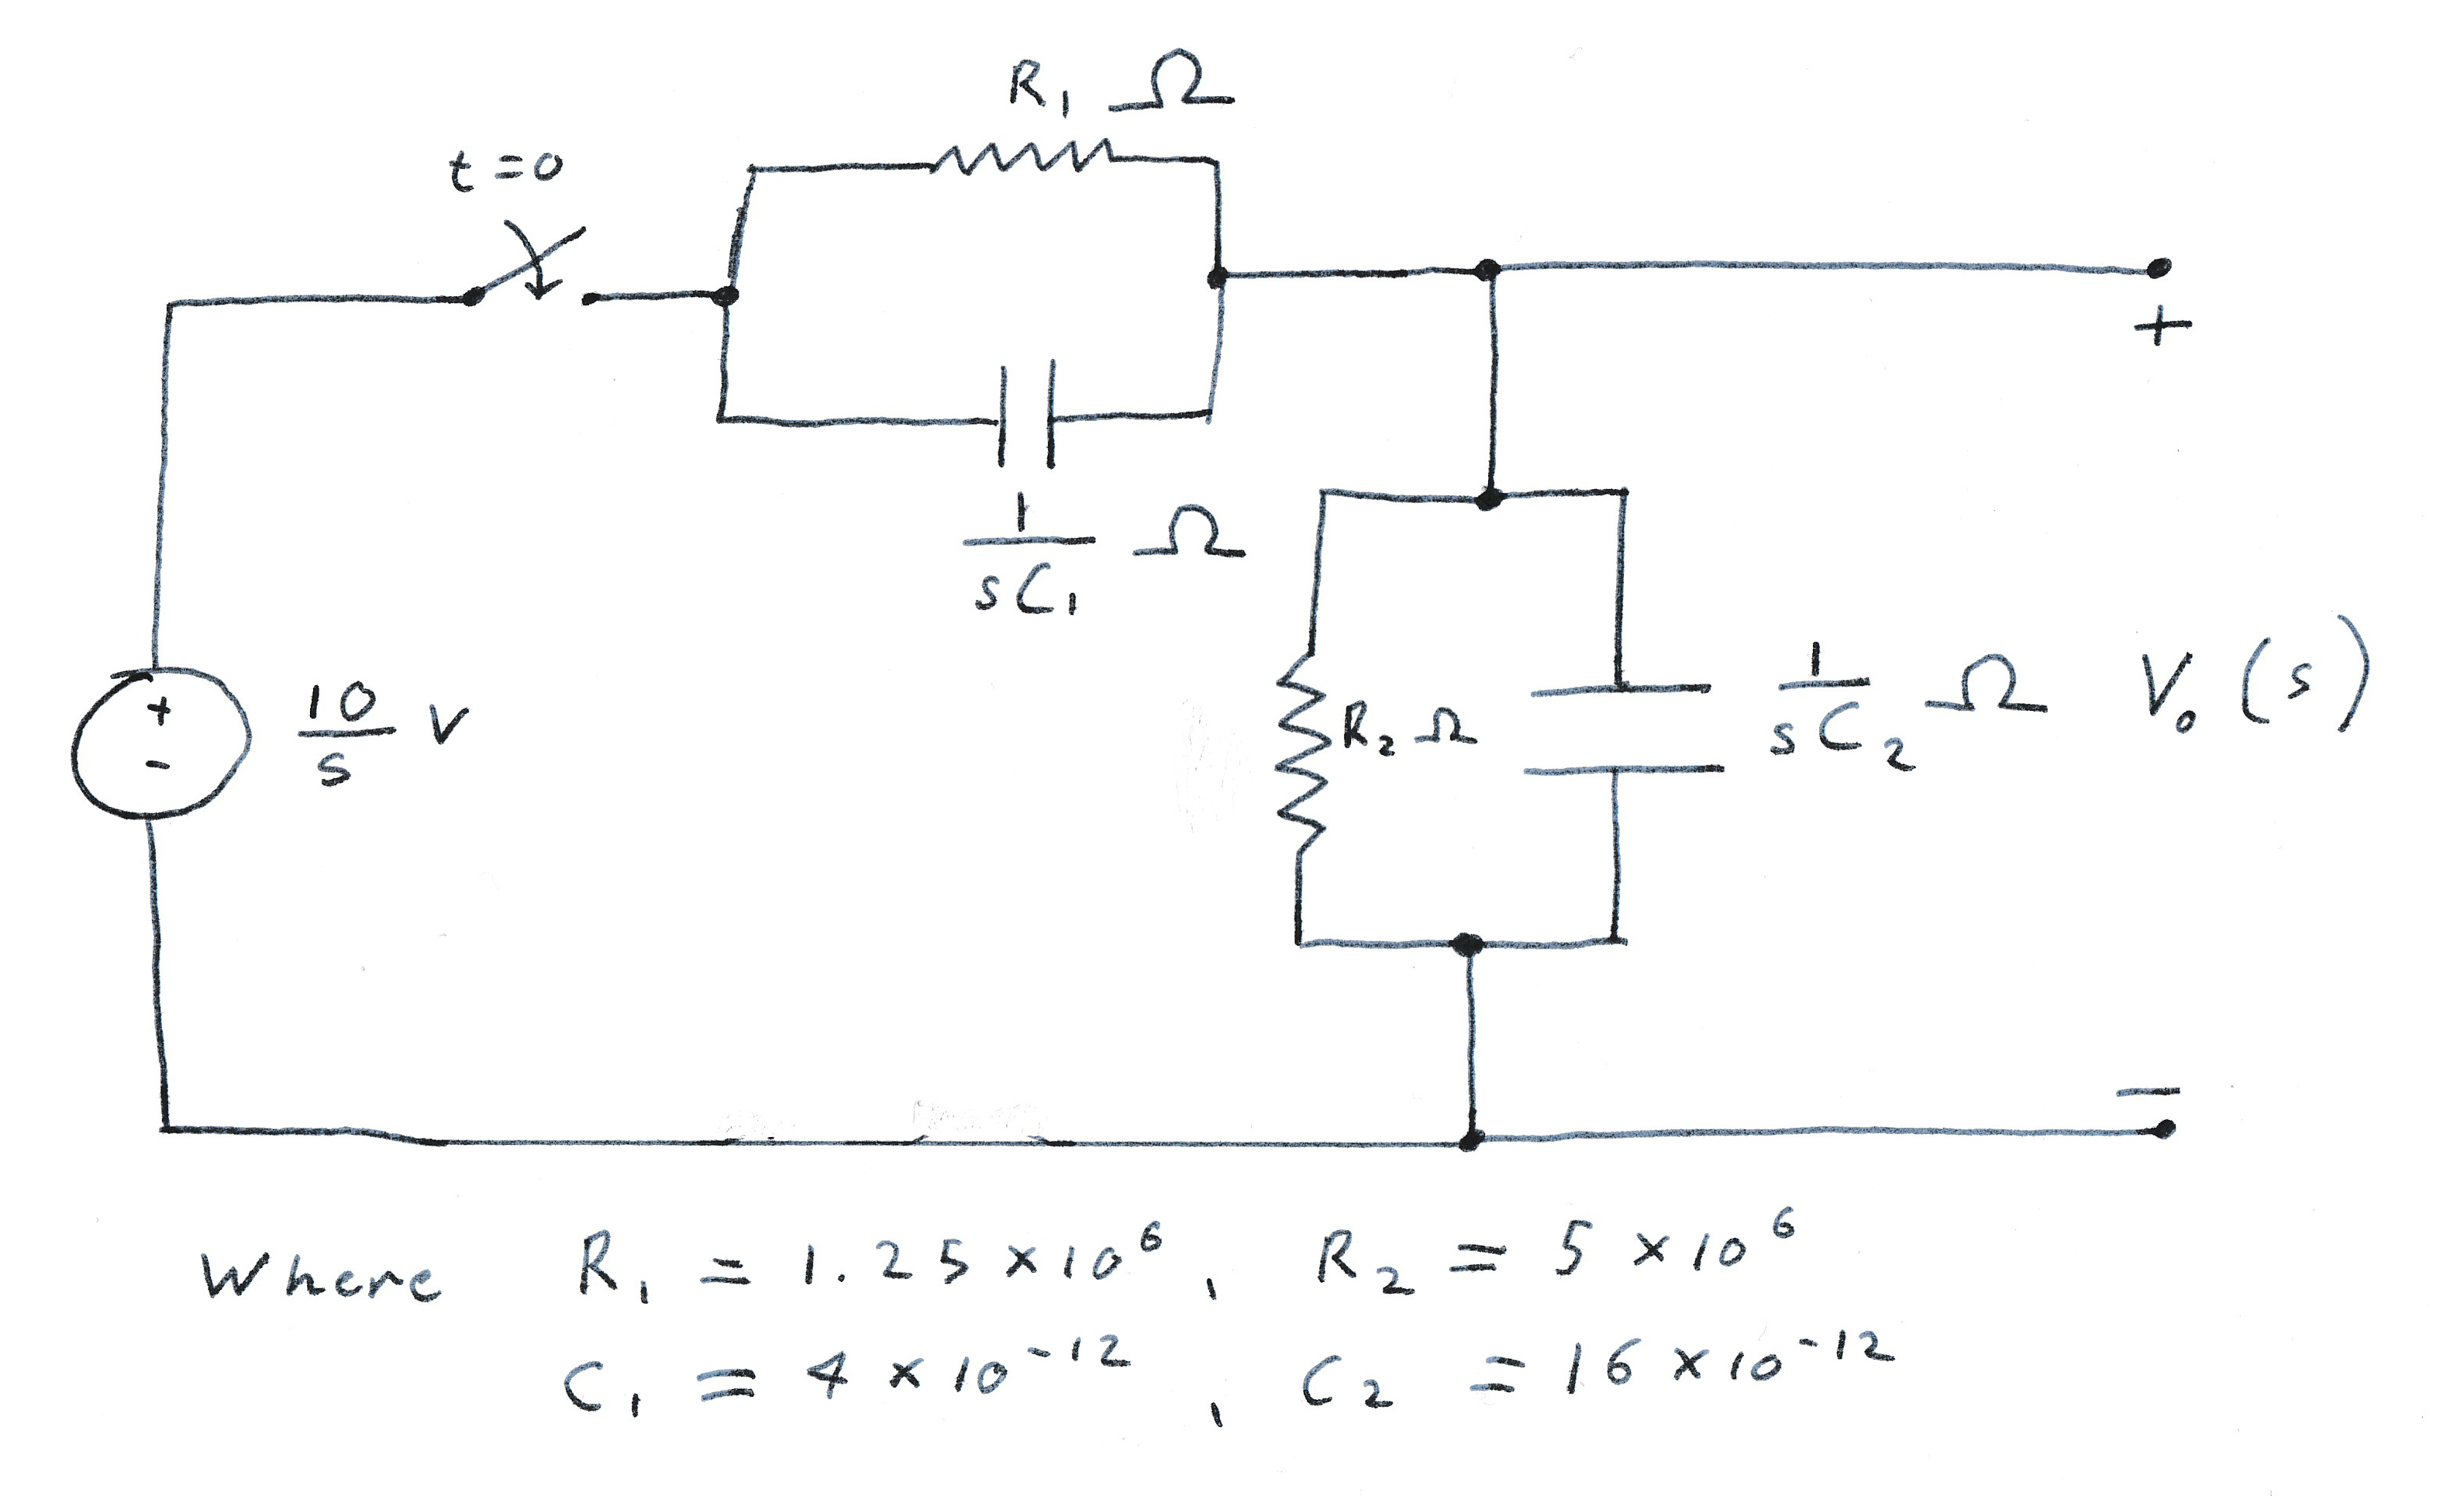
\includegraphics[scale=0.75]{1a.JPG}
		\end{center}
		\end{figure}
	}
	\item{
	%Part b
		\begin{align*}
		Z_{eq1} &= \left( \frac{1}{Z_{R_1}} +								%NEXTLINE
		\frac{1}{Z_{C_1}} \right)^{-1}\\
		&= \left( \frac{1}{R_1} + \frac{1}{\dfrac{1}{sC_1} } \right)^{-1}\\
		&= \left(\frac{1}{1.25 \times 10^6} + 								%NEXTLINE
		s \cdot 4 \times 10^{-12}\right)^{-1} \Omega\\
		&= \left(\frac{1 + 1.25\times 10^6 \cdot (s \cdot 4 \times 10^{-12})%NEXTLINE
		}{ 1.25\times 10^6} \right)^{-1} \; \Omega\\
		&= \frac{1.25\times 10^6}{1 + 1.25\times 10^6 						%NEXTLINE
		\cdot (s \cdot 4 \times 10^{-12})} \; \Omega\\
		&= \frac{2.5 \times 10^{11}}{s + 2 \times 10^5} \; \Omega
		\end{align*}
	}
	\item{
	%Part c
		\begin{align*}
		Z_{eq2} &= \left( \frac{1}{Z_{R_2}} +								%NEXTLINE
		\frac{1}{Z_{C_2}} \right)^{-1}\\
		&= \left( \frac{1}{R_2} + \frac{1}{\dfrac{1}{sC_2} } \right)^{-1}\\
		&= \left( \frac{1}{5\times 10^6} +									%NEXTLINE
		s \cdot 16 \times 10^{-12} \right)^{-1} \; \Omega\\
		&= \left( \frac{1 + 5\times 10^6 \cdot								%NEXTLINE
		(s \cdot 16 \times 10^{-12})}{5\times 10^6} \right)^{-1} \; \Omega\\
		&= \frac{5 \times 10^6}{1 + 5\times 10^6 							%NEXTLINE
		\cdot(s \cdot 16 \times 10^{-12})} \; \Omega \\
		&= \frac{6.25 \times 10^{10}}{s + 1.25 \times 10^4} \; A
		\end{align*}
	}
	\item{
	%Part d
		Using voltage division:
		\begin{align*}
		V_o(s) &= V_{in}(s) \cdot \frac{Z_{eq2}}{Z_{eq1} + Z_{eq2}}\\
		&= \frac{10}{s} \cdot \frac{\dfrac{6.25 \times 10^{10}}				%NEXTLINE
		{s + 1.25 \times 10^4}}{\dfrac{6.25 \times 10^{10}}					%NEXTLINE
		{s + 1.25 \times 10^4} + \dfrac{2.5 \times 10^{11}}					%NEXTLINE
		{s + 2 \times 10^5}} \; V\\
		&= \frac{10}{s} \cdot \frac{\dfrac{6.25 \times 10^{10}}             %NEXTLINE
		{s+1.25 \times 10^4}}{\dfrac{(6.25 \times 10^{10})					%NEXTLINE
		(s + 2\times 10^5) + (2.5 \times 10^{11})(s + 1.25 \times 10^4)}	%NEXTLINE
		{(s + 1.25 \times 10^4)\cdot(s + 2 \times 10^5)}} \; V\\
		&= \frac{10}{s} \cdot \frac{6.25 \times 10^{10}}            
		{s+1.25 \times 10^4} \cdot \frac{(s + 1.25 \times 10^4)
		\cdot(s + 2 \times 10^5)}{(6.25 \times 10^{10})
		(s + 2\times 10^5) + (2.5 \times 10^{11})
		(s + 1.25 \times 10^4)} \; V\\
		&= \frac{6.25 \times 10^{11} \cdot (s + 1.25 \times 10^4) \cdot 
		(s + 2 \times 10^5)}{3.125 \times 10^{11} \cdot s \cdot 
		(s + 1.25 \times 10^4) \cdot (s + 5 \times 10^4)} \; V\\
		&= \frac{2 \cdot (s + 2 \times 10^5)}
		{s \cdot (s + 5 \times 10^4)} \; V\\
		&= \frac{2s + 4 \times 10^5}{s^2 + 5 \times 10^4 \cdot s} \; V\\
		\end{align*}
		Using Partial fractions to continue.
		\begin{align*}
		\frac{2s + 4 \times 10^5}{s^2 + 5 \times 10^4 \cdot s} &= 
		\frac{A}{s} + \frac{B}{50000}\\
		A(s+50000) + Bs &= 2(s + 200000)\\
		(s = 0): \; 50000A &= 400000\\
		\implies A &= 8\\
		(s = -50000): \;  -50000B &= 300000\\
		B &= -6\\
		\implies V_o(s) = \frac{8}{s} - \frac{6}{s + 50000} \; V
		\end{align*}
		Using inverse Laplace transform to find $v_o(t)$.
		\begin{align*}
		v_o(t) &= \mathcal{L}^{-1} [V_o(s)]\\
		&= \mathcal{L}^{-1} \left[\frac{8}{s} - \frac{6}{s + 50000}\right]\; V\\
		&= (8 -6 e^{-50000t})u(t)\;V
		\end{align*}
	}
	\item{
	%Part e
		Using Ohm's Law in frequency domain:
		\begin{align*}
		V_{in}(s) &= Z_{eq} \cdot I_o(s)\\
		&= (Z_{eq1} + Z_{eq2}) \cdot I_o(s)\\
		\implies I_o(s) &= \frac{V_{in}(s)}{Z_{eq1} + Z_{eq2}}\\
		&= \frac{\dfrac{10}{s}} 
		{\dfrac{2.5 \times 10^{11}}
		{s + 2 \times 10^5} + \dfrac{6.25 \times 10^{10}}{s + 1.25 \times 10^4}} \; A\\
		&= \frac{\dfrac{10}{s}} 
		{\dfrac{3.125 \times 10^{11} \cdot (s + 50000)}{(s+12500)\cdot(s+200000)}} \; A\\
		&= \frac{(s+\sx)\cdot(s+\sy)}{\sz \cdot s \cdot (s + \sw)} \; A\\
		&= \frac{s^2 + s(\sx + \sy) (\sx)(\sy)}
		{\sz \cdot s^2 + s(\sz)(\sw)}\\
		&= \frac{\dfrac{s^2}{\sz} + s \dfrac{\sx + \sy}{\sz} + \dfrac{(\sx)(\sy)}{\sz}}{s^2 + s (\sw)}\\
		&= \frac{1}{\sz} + \frac{s\left(\dfrac{\sx+\sy-\sw}{\sz}\right) + \dfrac{(\sx)(\sy)}{\sz}}{s(s+\sw)}\\
		&= \frac{1}{\sz} + \frac{s \cdot \dfrac{13}{2500000} + \dfrac{2}{25} }{s(s+\sw)} 
		\end{align*}
		Use partial fraction expansion on the s term:
		
		\begin{align*}
		&\frac{A}{s} + \frac{B}{s + \sc} = \frac{\sa \cdot s + \sb}{s(s + \sc)}\\
		\implies &A(s + \sc) + B(s) = \sa \cdot s + \sb\\
		(s = 0) \implies &A \cdot \sc = \sb\\
		\implies &A = \frac{1}{625000}\\
		(s = -\sc) \implies &B(-\sc) = -\left(\sa\right)(\sc) + \sb\\
		\implies &B = \left( \sa \right) - \frac{\sb}{\sc}\\
		\implies &B = \frac{9}{2500000}
		\end{align*}				
			
		\begin{align*}
		\implies I_o(s) &= \frac{9}{2500000 \cdot(s+50000)} + \frac{1}{625000 \cdot s} 
		+ \frac{1}{3.125 \times 10^{10}} \; A
		\end{align*}
		Using inverse Laplace transform to find $i_o(t)$.
		\begin{align*}
		i_o(t) &= \mathcal{L}^{-1}\left[ I_o(s) \right]\\
		&= \mathcal{L}^{-1} \left[ \frac{9}{2500000 \cdot(s+50000)} 
		+ \frac{1}{625000 \cdot s} + \frac{1}{3.125 \times 10^{10}} \right]\\
		&= 3.6 \times 10^{-6} e^{-50000t} \cdot u(t) + 1.6 \times 10^{-6} \cdot u(t) + 3.2 \times 10^{-11} \delta(t) \; A
		\end{align*}
		If we assume $t>0$ only then:
		$$ i_o(t) = (3.6 \cdot e^{-50000t} + 1.6) \; \mu A $$
	}
\end{enumerate}
		}
		\item{
		%Question 2
		\let\clearpage\relax
		Q2

\begin{enumerate}
	\item{
	%Part a
	}
	\item{
	%Part b
	}
	\item{
	%Part c
	}
\end{enumerate}
		}
		\item{
		%Question 3
		\let\clearpage\relax
		\begin{enumerate}
	\item{
	%Part a
		Convert circuit to its s domain equivalent, and assume no energy stored at $t=0^-$:
		\begin{figure}[H]
			\centering
			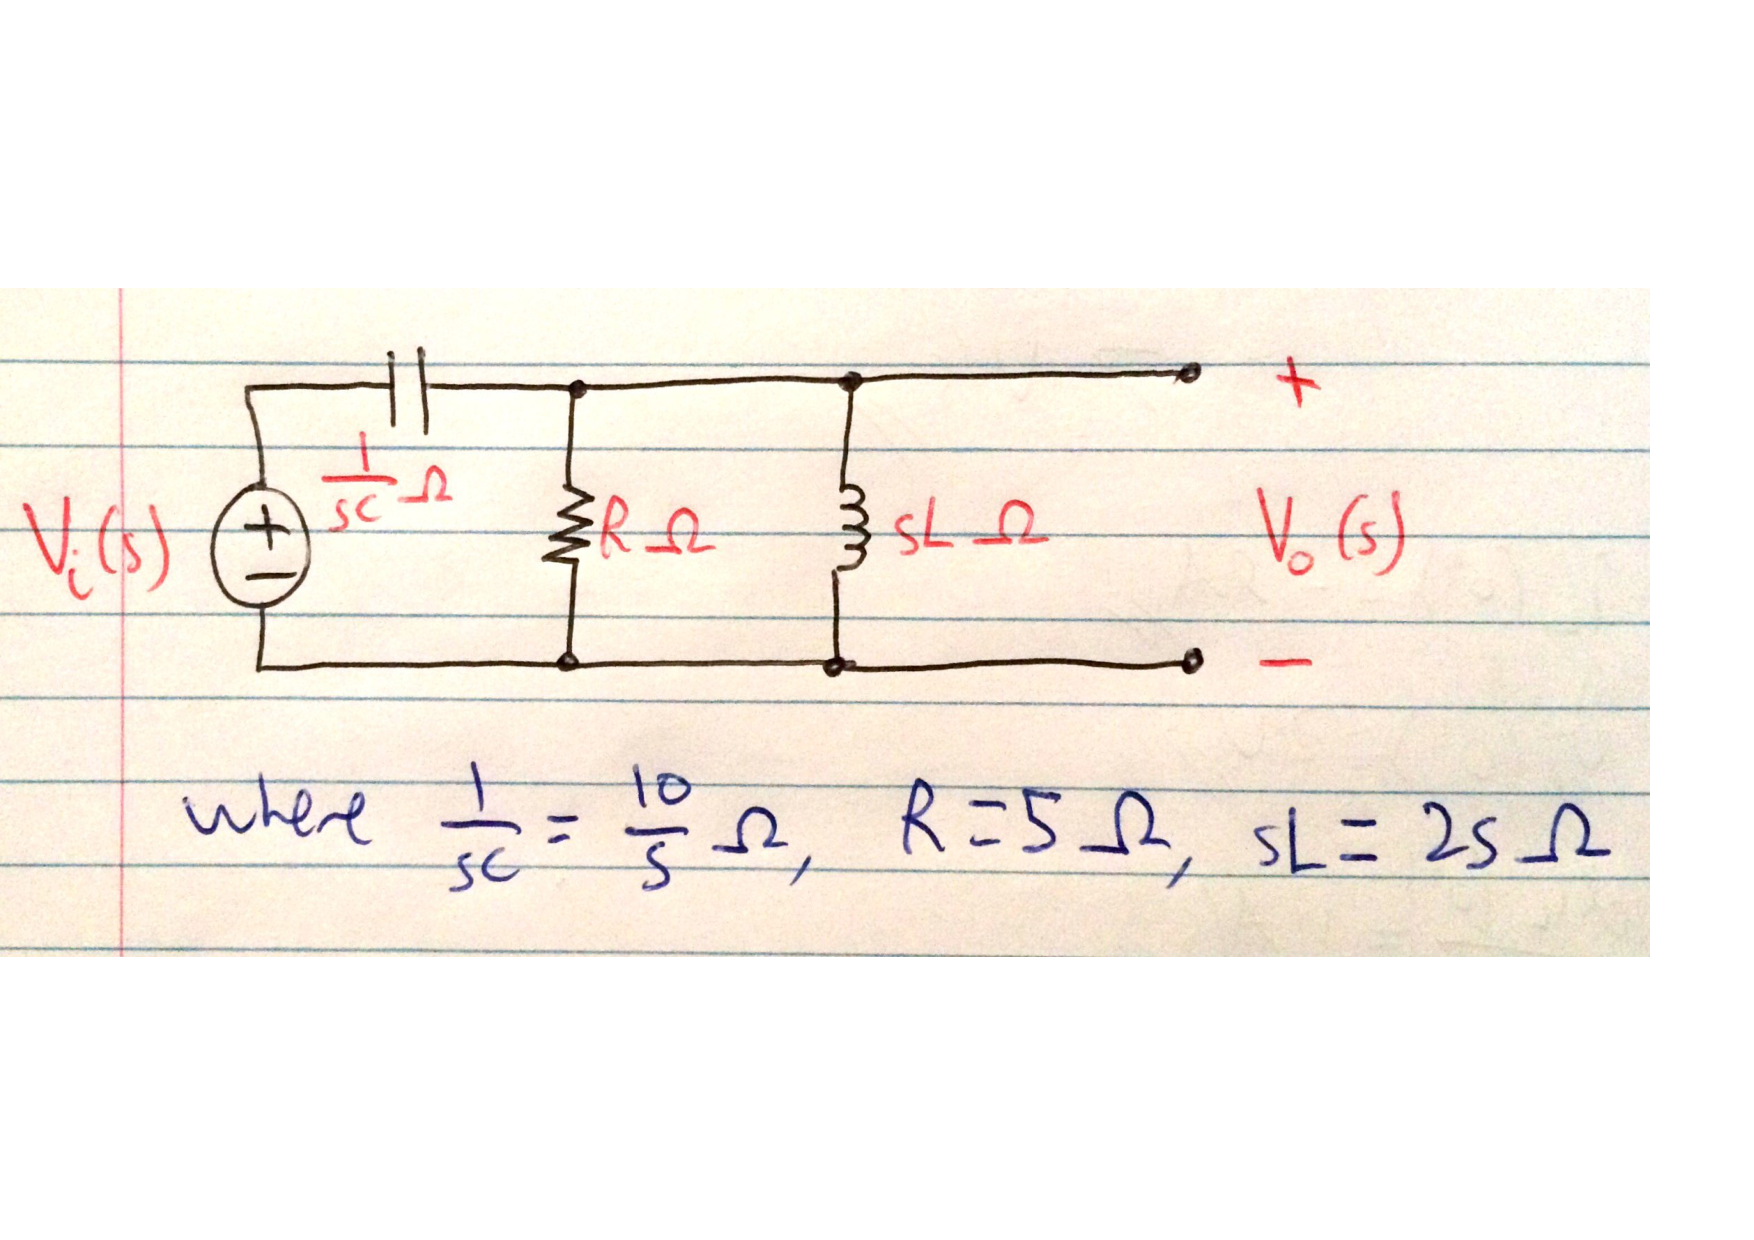
\includegraphics[scale=0.55]{q3a.pdf}
		\end{figure}
		Find $V_o(s)$ by recognising circuit is a voltage divider:
		\begin{align*}
			V_o(s) &= V_i(s) \times \frac{\frac{5\times2s}{5+2s}}{\frac{5\times2s}{5+2s} + \frac{10}{s}} \\ 
			\\
			\therefore H(s) &= \frac{10s}{10s+ \frac{50}{s} + 20} \\
			&= \frac{10s^2}{10s^2+20s+50} \\
			\\
			\therefore H(s) &= \frac{s^2}{s^2+2s+5}
		\end{align*}
		\\
	}

	\item{
	%Part b
		We note that the steady state response to the sinusoidal input will be given by the following equation:
		\begin{equation*}
			v_{oSS}(t) = 10 \times |H(j20)| \cos(20t + \theta(20))
		\end{equation*}
		\\
		Where $H(j\omega) = |H(j\omega)|e^{j\theta(\omega)}$
		\\ \\
		Therefore, find $|H(j20)|$ and $\theta(20)$:
		\begin{align*}
			H(j20) &= \frac{-400}{-395+j40} \\
			\\
			\therefore |H(j20)| &= \frac{400}{\sqrt{(-395)^2+40^2}} \\
			&= 1.008
		\end{align*}
		\begin{align*}
			\mathrm{And} \ \theta(20) &= \arctan \left(\frac{0}{-400} \right) - \arctan \left(\frac{40}{-395} \right) \\
			&= 180\degree - 174.22\degree \\
			&= 5.78\degree
		\end{align*}
		Finally sub these values into the equation for $v_{oSS}$:
		\begin{equation*}
			v_{oSS}(t) = 10.075 \cos(20t+5.78\degree) \ \mathrm{V}
		\end{equation*}
		\\
	}

\end{enumerate}

		}
		\item{
		%Question 4
		\let\clearpage\relax
		Start by converting the output response equation to its s-domain equivalent:
\begin{align*}
	V_o(s) &= \mathcal{L}[v_o(t)] \\
	&= \frac{10}{s+3} - \frac{20}{s+4} + \frac{10}{s+5} \\
	&= \frac{10(s+4)(s+5) - 20(s+3)(s+5) + 10(s+3)(s+4)}{(s+3)(s+4)(s+5)} \\
	&= \frac{20}{(s+3)(s+4)(s+5)}
\end{align*}
Now by definition, $V_i(s) = \frac{V_o(s)}{H(s)}$, therefore:
\begin{align*}
	V_i(s) &= \frac{20}{(s+3)(s+4)(s+5)} * \frac{(s+3)(s+4)}{2(s+5)} \\
	&= \frac{10}{(s+5)^2}
\end{align*}
Now convert the input function back to the time domain:
\begin{align*}
	v_i(t) &= \mathcal{L}^{-1}[V_i(s)] \\
	&= 10te^{-5t} u(t) \ \mathrm{V}
\end{align*}

		}
		\item{
		%Question 5
		\let\clearpage\relax
		\begin{enumerate}
	\item{
	%Part a
		\begin{align*}
			F(s) &= \frac{20s^2+141s+315}{s \left(s^2+10s+21 \right)} \\
			&= \frac{20s^2+141s+315}{s(s+7)(s+3)} \\
		\end{align*}
		Perform partial fraction expansion:
		\begin{equation*}
			\frac{20s^2+141s+315}{s(s+7)(s+3)} = \frac{A}{s} + \frac{B}{s+7} + \frac{C}{s+3}
		\end{equation*}
		\begin{equation*}
			\therefore 20s^2+141s+315 = A(s+7)(s+3) + Bs(s+3) + Cs(s+7)
		\end{equation*}
		Now solve for A, B and C:
		\begin{equation*}
			s = 0 \implies 315 = A(7)(3) \implies A = 15
		\end{equation*}
		\begin{equation*}
			s = -7 \implies 308 = B(-7)(-4) \implies B = 11
		\end{equation*}
		\begin{equation*}
			s = -3 \implies 72 = A(-3)(4) \implies C = -6
		\end{equation*}
		And we arrive at $F(s)$ in partial fraction expanded form:
		\begin{equation*}
			F(s) = \frac{15}{s} + \frac{11}{s+7} - \frac{6}{s+3}
		\end{equation*}
		Now perform the inverse Laplace transform:
		\begin{align*}
			f(t) &= \mathcal{L}^{-1}[F(s)] \\
			&= \left(15 + 11e^{-7t} - 6e^{-3t} \right) u(t) \ \mathrm{V}
		\end{align*}
	}
	\item{
	%Part b	
	}
	\item{
	%Part c	
	}
	
\end{enumerate}

		}
		
		\item{
		%Question 6
		\let\clearpage\relax
		Q6
		}
	\end{enumerate}

\end{document}
